\documentclass[letterpaper]{article}
\usepackage[submission]{aaai2027}
\usepackage[hyphens]{url}
\usepackage{graphicx}
\urlstyle{rm}
\def\UrlFont{\rm}
\usepackage{natbib}
\usepackage{caption}
\frenchspacing
\usepackage{amsmath,amssymb,amsthm,booktabs,tabularx,array}
\pdfinfo{/TemplateVersion (2027.1)}
\setcounter{secnumdepth}{2}
\newtheorem{theorem}{Theorem}
\newcommand{\code}[1]{\texttt{#1}}
\title{TrustBound: A Mechanized Note on Payment-Epoch Completeness}
\author{Anonymous Submission}
\affiliations{}
\begin{document}
\maketitle
\begin{abstract}
A payment receipt establishes an observed outcome; exact epoch closure also
requires complete accounting and exclusion of later effects under earlier
authority. This note makes those obligations explicit for request-only agents
using a trusted payment service. In a Lean transition model, recording before
granting authority and serializing both with an admission fence derive a fixed
journal covering effects and remaining rights. Complete source-side discharge
establishes future stability; truthful per-identity outcomes additionally
establish exact identity-level accounting. A constrained provider model permits
unregistered inert objects while mediating every activation. Reproduction checks
14 exported results and rejects eight premise-removal mutations. A finite
diagnostic, whose two strong comparator labels share the same fence-and-contiguity
acceptance rule, documents the evidence boundary; a small flight--hotel example
separates payment closure from commit-time policy and trip usability.
The contribution is an auditable assumption contract, a checked construction,
and reproducible examples that specialize existing closure and authorization
principles to payment epochs.
\end{abstract}

\section{Introduction}
A travel business may delegate flight and hotel booking to separate agents.
A flight payment can be known while a hotel payment has an uncertain response.
The service may stop admitting new work while the earlier hotel request remains
able to execute. Booking completion, a balanced reservation ledger, and a signed
list of observed payments each leave a question unanswered: is the relevant
payment history complete and unable to grow under earlier authority?

This paper fixes one merchant payment path and epoch. Agents are request
proposers; the service, its journal, and the relevant source contracts are
trusted. Travel is a motivating application, not a claim of verified composition
across booking providers or independent issuers. Removing an itinerary
coordinator does not remove trust in the payment authority.

\paragraph{Objective and operational meaning.}
The goal is an auditable criterion for closing one agent-initiated payment epoch:
every in-scope effect identity is accounted for and no remaining authority can
produce another such effect. Running the artifact checks this conditional model,
its premise-sensitive proofs, and a finite evidence diagnostic. It produces a
reproduction report, not a closure certificate for a merchant. For a flight--hotel
request pair, an earlier hotel payment that can still execute prevents closure;
an unknown past outcome prevents exact accounting even after execution stops.
Applying the criterion requires the deployment to satisfy A1--A5 and a justified
mapping of its effects and rights to the model.

\paragraph{Why this scope.}
Authenticating separate parties' reports establishes their origin, not that
their combined contents cover every in-scope effect or remaining right. In the
restricted view of our bypass diagnostic, an execution with an omitted effect
and one without it supply identical evidence. An auditor restricted to that
evidence cannot accept one as complete while rejecting the other. This motivates
an explicit coverage contract rather than treating signatures as a substitute
for it, consistent with the mediation and boundary-adequacy requirements in
Salas and EffectBound~\citep{salas,effectbound}. Section~\ref{sec:diagnostic}
also records the withdrawal of a 27 October comparison that exposed a hidden
effect flag to the verifier. That methodological correction removed a purported
advantage; it is not evidence of a general impossibility theorem. Richer
observations or enforceable coverage contracts may distinguish the executions.
The note therefore fixes one mediated service and makes coverage, terminality
and export obligations explicit, rather than inferring cross-party completeness
from authentic reports alone.

The contribution is assumption hygiene: A1--A5 separate operational trust
premises from the ordering and coverage facts derived by the model. Two small
Lean modules and eight premise-removal checks make the boundary inspectable.
The checks expose dependence of the supplied proofs, rather than establish a
minimal or sufficient real-provider contract. Effect closure, commit-time
validation, and mediation already have close formal treatments
\citep{effectbound,cta,salas}; this note supplies a payment-epoch specialization
and a reproducible artifact. Section~\ref{sec:related} positions that artifact
against the nearest work.

\section{Scope and observation contract}
\label{sec:scope}
\subsection{Trusted-service assumptions}
Agents may replay, reorder, forge, or omit requests, but cannot access the
service machine, payment keys, journal, or privileged controls. The prototype's
request interface accepts previously approved command identities and limited
status/reconciliation requests. General approval and multi-tenant authorization
are outside this evaluation.

The epoch's economic scope must be fixed before execution. A second credential,
operator, or automation that can create an attributable effect is an in-scope
route to mediate, not a reason to redefine the scope after observing an effect.
Recovery of an admitted request remains part of its execution authority.
The modeled epoch starts empty. Applying the theorem to a new epoch therefore
requires that no earlier right or effect attributable to that epoch is omitted
from the initial abstraction. Resetting a journal or relabeling a delayed
request does not meet this requirement. Importing pre-existing work would
require an explicitly justified initial-state invariant, which is not provided
by the empty-start theorem here.

\begin{description}
\item[A1: Request-only agents.] Agents have no access to the trusted service's
internals or administration. Same-host arbitrary-code adversaries are excluded.
\item[A2: Exclusive scoped activation.] Every effect-capable route in the
predefined epoch is mediated. Identities cannot be reassigned to evade the fence.
\item[A3: Durable ordered service.] Recording precedes authority, recording
and grants serialize with the fence, and committed state cannot roll back.
\item[A4: Truthful source terminality.] Outcomes bind the correct identities
and facts. Discharge irreversibly removes all remaining effective authority,
including in-flight delivery and provider recovery.
\item[A5: Faithful complete export.] The auditor receives the authoritative
journal and truthful outcomes for the same declared scope and cut.
\end{description}


A1 does not imply A2. The state machines enforce abstract ordering in A3; no
refinement from executable Python and storage to those machines is proved.
A4 is a semantic source contract, not a conclusion from a terminal-looking
client status. A signature authenticates an assertion without proving A5.
A separately obtained view from the same processor is not an independently
trusted issuer. Successful API tests do not establish these premises universally.
Agents need not trust one another's assertions. Trust is placed in the service's
enforcement and durable state and in the qualified provider evidence; the model
does not establish those parties' trustworthiness.



\subsection{Four different assertions}
\emph{Admission closed} means no new records or grants are accepted. Earlier
rights may still execute. \emph{Exposure covered} means retained liability
covers possible cumulative debits; an uncertain operation can meet a bound
without a known outcome. \emph{Execution stopped} means no permitted
continuation adds an attributable effect, although past effects may remain
unknown to the observer. \emph{Exactly closed} combines complete accounting
of the admitted population with exclusion of future effects.

These assertions are specialized to an exact-accounting question. EffectBound
already separates future-use closure, policy-relative effect closure, and
quiescence~\citep{effectbound}. Its policy-relative effect closure can permit
continued safe work, whereas our execution-stopped assertion excludes any new
in-scope modeled effect.

Our main theorem concerns effect identities. It does not establish booking
success, legal finality, eventual completion, or a net balance immune to refunds
and disputes. Separate amount and dispatch models in the research workspace
are not composed into an end-to-end monetary theorem here.



\section{Admission, fencing, and exact closure}
\label{sec:theorem}
\subsection{State and transitions}
The Lean state is $(J,I,R,E,F)$: the journal, issued identities, remaining
effective rights, effect history, and closed flag. The first four components
are lists of natural-number identities; the initial lists are empty and $F$ is
false. Set notation below abbreviates list membership, except that history
equality is actual list equality. $R$ includes external delivery authority,
not merely the client's queue. $E$ is ghost history, not an auditor input.

\begin{table}[ht]
\centering
\begin{tabularx}{\linewidth}{@{}l X X@{}}
\toprule
Action & Guard & State change \\
\midrule
Record $i$ & $\neg F$, $i\notin J$ & Prepend $i$ to $J$. \\
Grant $i$ & $\neg F$, $i\in J$, $i\notin I$ & Prepend $i$ to $I$ and $R$. \\
Deliver $i$ & $i\in R$ & Remove $i$ from $R$; prepend it to $E$. \\
Cancel $i$ & No additional guard & Remove $i$ from $R$. \\
Fence & No additional guard & Set $F$ to true. \\
\bottomrule
\end{tabularx}
\caption{The admission model. Cancel removes current effective rights; it is
not an API cancellation acknowledgement or a permanent identity tombstone.
Unlisted fields are unchanged.}
\label{tab:steps}
\end{table}

All guards and updates in Table~\ref{tab:steps} are atomic abstract transitions.
The issued list prevents granting the same identity again. The model represents
one effect per identity, not arbitrary partial-capture or recovery lineages.
A finite run is the reflexive transitive closure of the transition relation.
The proofs place no finite bound on run length or on the identity domain.

Cancel does not add to $I$ or set a terminal flag. Recording $i$, cancelling it
before any grant, and then granting and delivering it is permitted while the
epoch is open. After a grant, $I$ prevents regrant; after a fence, all grants
are disabled. Thus a cancelled identity is not unconditionally terminal in
this model. Permanent terminal-identity exclusion is an additional rule of
the provider model in Section~\ref{sec:mapping}. Neither cancellation nor
discharge erases a past effect or represents a refund.


\subsection{Conditional theorem}
The proof is a direct induction on single transitions followed by disabling
effect-producing transitions after drainage; the note's value lies in the
explicit premises and mutation checks rather than proof complexity.
\begin{samepage}
\begin{theorem}[Fenced identity coverage and exact closure]
Let $s$ be reachable from the initial state with $F(s)=\mathrm{true}$, and let
$t$ be reachable from $s$ by any finite permitted run. Then
\begin{align}
J(t)&=J(s),\label{eq:fixed}\\
R(t)\cup E(t)&\subseteq J(s).\label{eq:covered}
\end{align}
If every $i\in J(s)$ is absent from $R(s)$ and a predicate $\mathrm{reported}$
satisfies $\mathrm{reported}(i)\Leftrightarrow i\in E(s)$ for all such $i$, then
\begin{align}
R(t)&=\varnothing,& E(t)&=E(s),\label{eq:stable}\\
i\in E(t)&\ \Longleftrightarrow\ i\in J(s)\land\mathrm{reported}(i).
\label{eq:exact}
\end{align}
\end{theorem}
\end{samepage}



\begin{proof}
Every transition preserves coverage $R\cup E\subseteq J$: a grant needs a
journal entry, delivery consumes an existing right, and cancellation introduces
no effect. Reachability from the empty state therefore establishes coverage.
After fencing, record and grant are disabled, so the journal is fixed. This
proves~\eqref{eq:fixed}--\eqref{eq:covered}. Coverage and discharge of every
journaled identity imply $R(s)=\varnothing$. No subsequent transition can
reintroduce rights or deliver an effect, yielding~\eqref{eq:stable}. Truthful
reports identify precisely the executed journal entries, giving~\eqref{eq:exact}.
\end{proof}


The checked declarations implement these four obligations.\footnote{\raggedright In
\code{Admission.lean}: \code{fenced\_population\_immutable},
\code{post\_fence\_coverage}, \code{drained\_fence\_effects\_stable}, and
\code{reconciled\_fence\_complete}.\par}
Future stability needs drainage but not an outcome report; exact identification
of the past additionally needs truthful reports. The theorem derives coverage
from guarded transitions. It does not discover whether every real route obeys
those transitions or whether a supplied export is faithful.
Truthful Boolean reports determine effect membership, not the historical
ordering of effects. The list equality states that the modeled history remains
unchanged; it does not reconstruct that ordering from the reports.

Figure~\ref{fig:completeness} separates future stability from knowledge of
past effects. Each multi-input conclusion requires all its incoming premises;
the arrows impose no temporal order on observations.

\begin{figure*}[t]
\centering
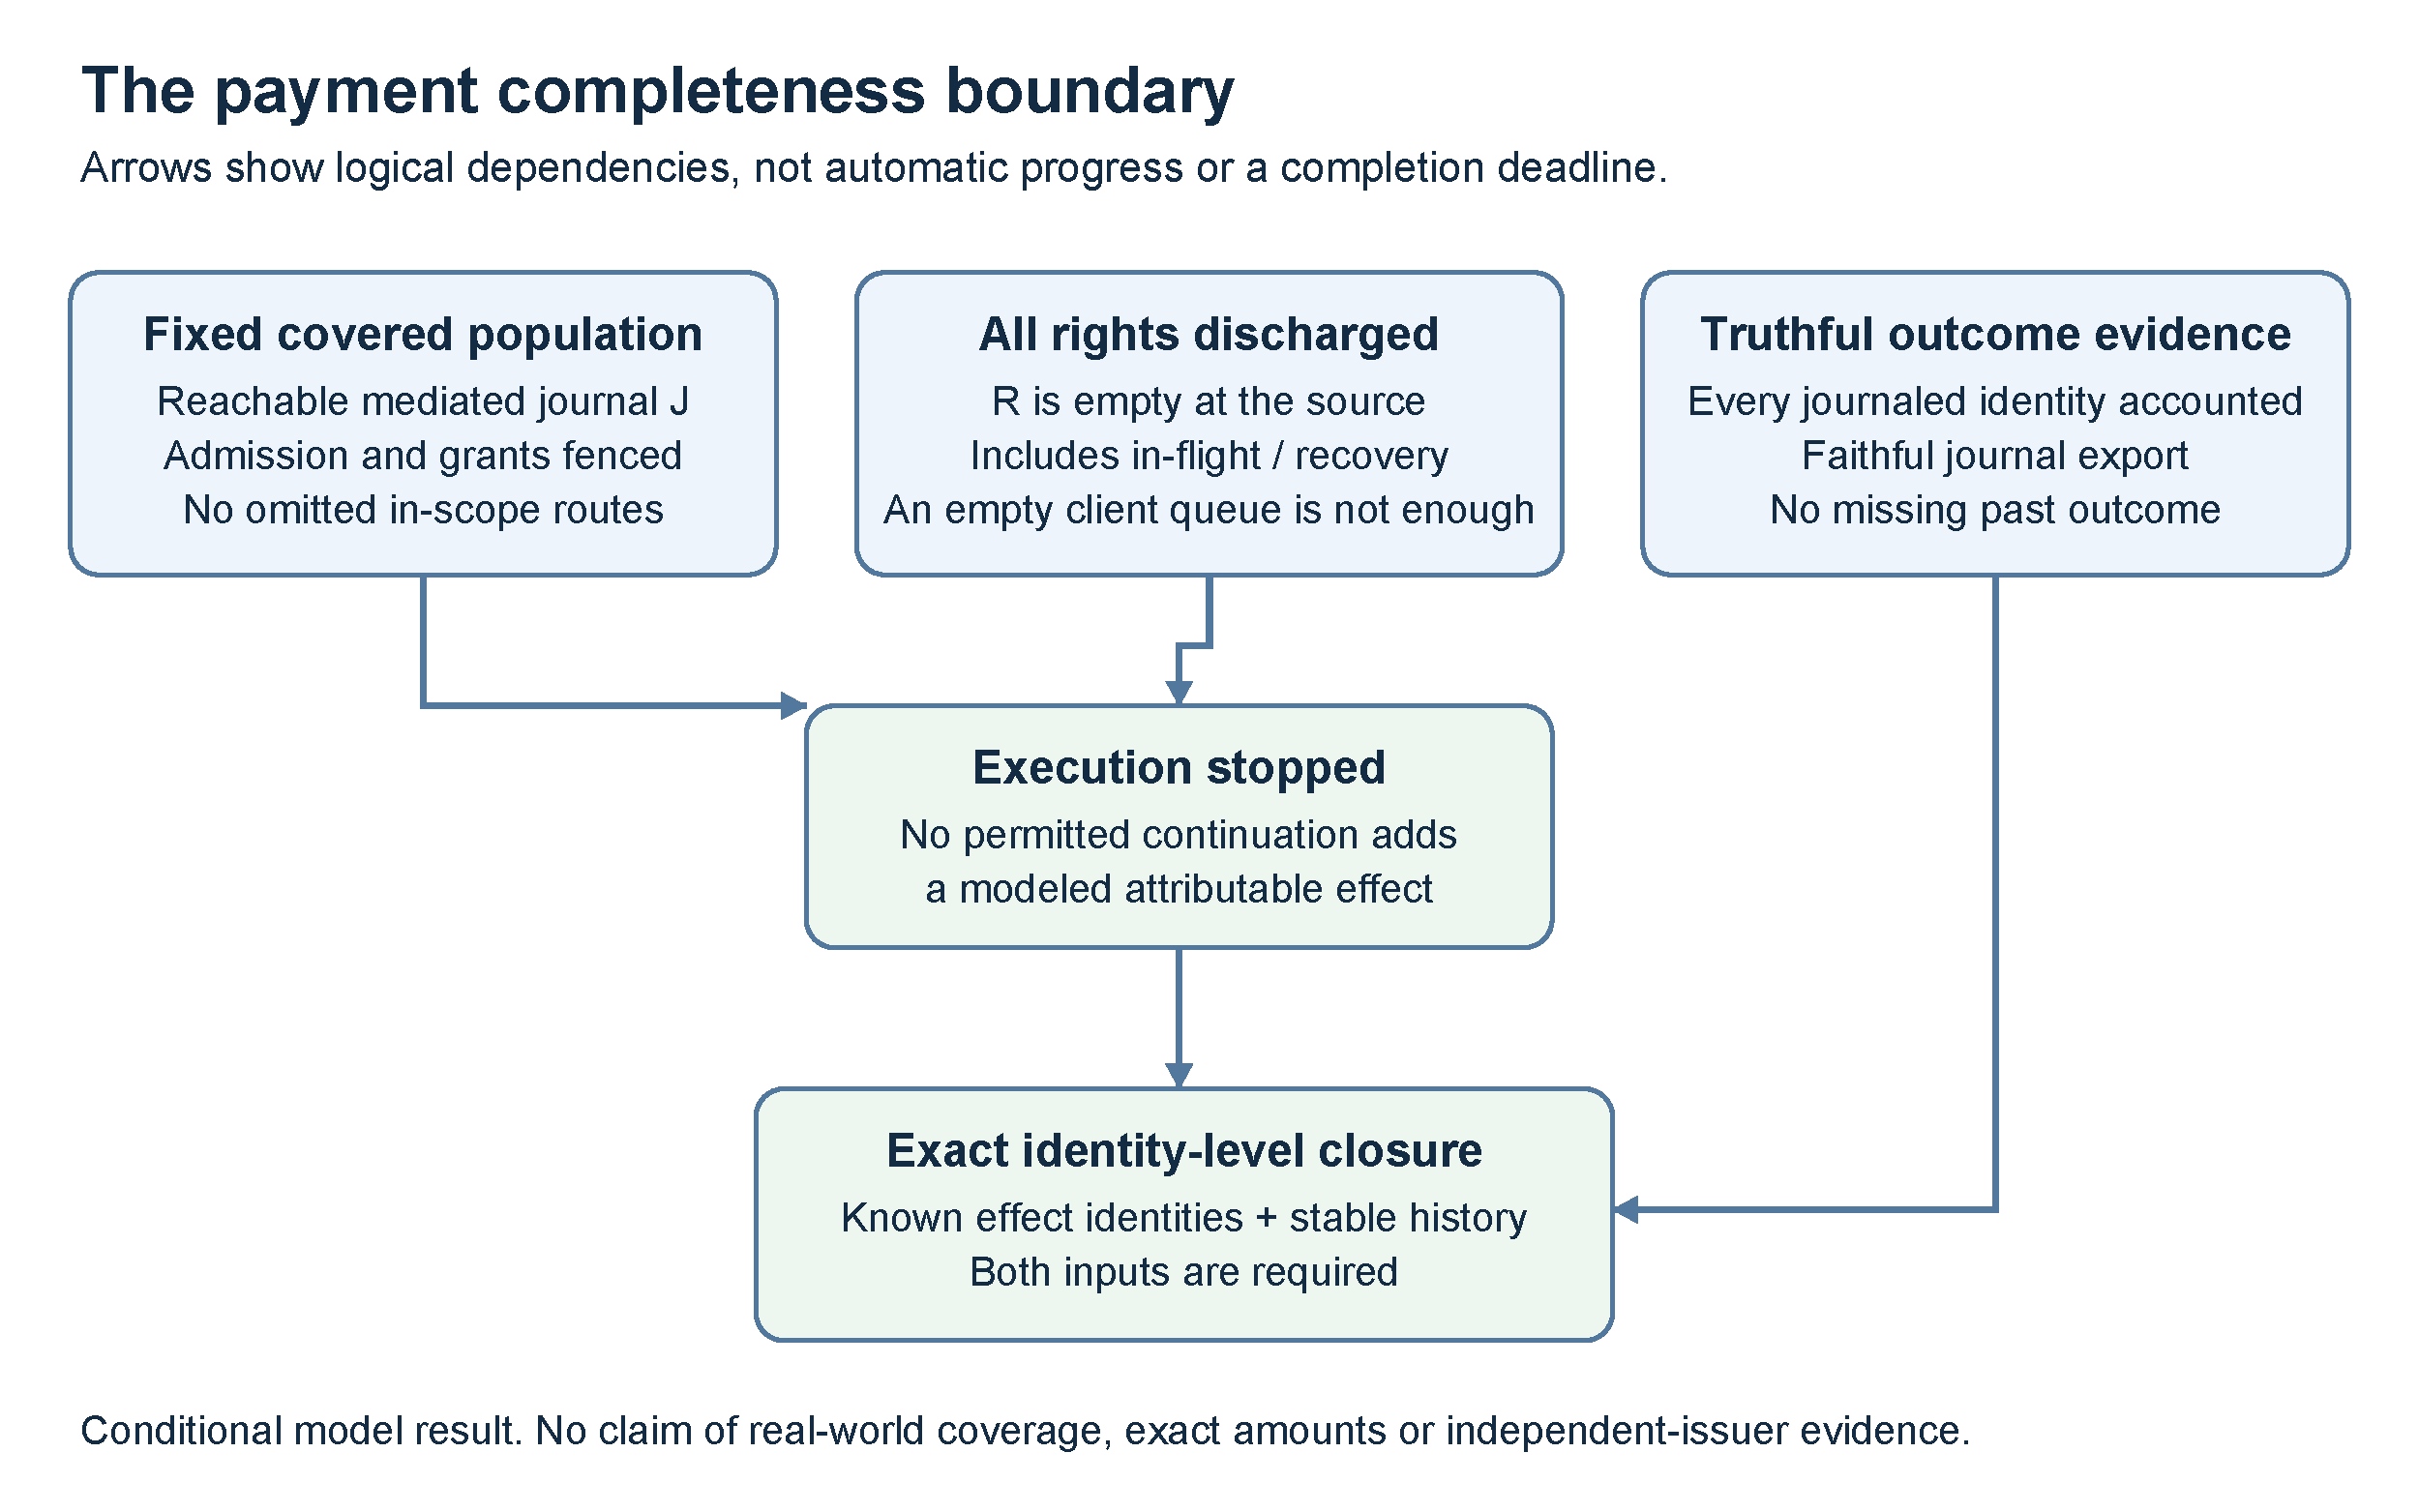
\includegraphics[width=\linewidth]{figures/completeness.pdf}
\caption{Logical dependencies of exact identity-level closure under the
specified transition rules. A fixed covered population, fenced admission and
grants, and discharge of all remaining effective rights yield future effect
stability. Truthful outcomes and a faithful complete export additionally identify
past effects. All incoming premises are required. The arrows express logical
dependence, not an observation order.}
\label{fig:completeness}
\end{figure*}

\subsection{Counterexecutions and transfer obligation}
The checked \code{fence\_without\_drain} execution records and grants an
identity, closes admission, and then delivers it. With a completed flight and
pending hotel operation, for example, $J=\{f,h\}$, $E=\{f\}$ and $R=\{h\}$.
Authorization may be safe while exact closure is false. This illustrates the same structural distinction as EffectBound's Kafka
applied-state fence, which leaves earlier authorized work able to append
\citep{effectbound}; our example is a model instance, not a new attack.

The checked \code{bypass\_breaks\_coverage} example adds an effect outside the
transition relation without changing the journal. This violates A2, rather
than disproving the theorem under its premises. Richer provider queries can
distinguish such histories; the example makes no full-API indistinguishability
claim.

The membership-only refinement bridge and its deployment obligations are stated in Appendix~\ref{app:bridge}.

\section{Constrained provider-contract mapping}
\label{sec:mapping}
The second model, \code{StripeGate.lean}, adds a collection of provider objects
and terminal identities around the admission state. Allocation creates an
inert object. Registration requires an existing object and an open epoch.
Dispatch requires registration, an open epoch, an unused identity, and absence
of terminal status. A paid transition consumes a right, records an effect,
and marks terminality. Cancellation removes the right and marks terminality.
Lost replies, reads, and rejected attempts can leave the model state unchanged;
any still-effective authority must remain represented in $R$.

\code{provider\_step\_refines} and \code{provider\_runs\_refine} map these
specified transitions to the admission model. Reachability then implies that
an unregistered object has neither a right nor an effect.
\code{terminal\_manifest\_drains} establishes an empty rights list when all
journal entries are terminal. After a fence, \code{terminal\_cut\_stable}
gives history stability. Terminality here is defined by permanent exclusion
of future effects, not inferred from a status name.

The practical motivation is an unconfirmed object with manual confirmation
and capture, durably registered before activation. Unknown inert objects need
not be enumerated to cover payments. The hard obligation is showing that
another credential, operator, automation, or configuration cannot activate one.
A lost creation response is harmless only under this inert-creation contract.
This is a model-to-model mapping, not verification of Stripe's servers or an adapter. AcquireBound already
separates acquisition from current-state activation and effect authority
\citep{acquirebound}; the inert-object mapping here specializes that separation.
Allocation can remain possible after a fence without invalidating the result:
registration and activation for that epoch are blocked. Conversely, a single
concrete operation that can debit more than once or create separately effective
descendants cannot be mapped to one modeled identity merely by sharing a
request identifier. Its effect granularity and remaining authority need a
separate justified representation; this paper supplies no such mapping.

\section{Evaluation and reproduction}
\label{sec:eval}
We separate fresh checks of the selected core from historical observations.
On 5 November 2026, a source-isolated run copied eight selected source and
configuration files, using existing Lean 4.19.0, Python 3.12.14, and pytest 9.0.2
installations. It made no provider requests. The release artifact was also
extracted into a separate directory and its included runner was executed there
with the same installed tools. Neither check was an independent clean-machine
installation or a real-deployment verification.

A separate 6 November export check repeated the selected core and the local
simulator successfully; implementation-suite details are in Appendix~\ref{app:artifact}.
On 7 November, rerunning the extracted selected-core archive reproduced the
same core totals with existing tools and no provider requests.

\subsection{Formal checks}
All eight exported admission results and all six provider-contract results
passed. Their accepted axiom reports use only \code{propext} and
\code{Quot.sound}, or no axioms; no custom axiom or unfinished proof is accepted.
The provider checker recompiles its admission dependency, which is not counted
as eight additional results.
The 14 exports include invariant and mapping results, two counterexecution
statements, and a conditional transfer bridge; they are not 14 independent
security guarantees. The two Lean modules use sequential atomic abstract
steps. Arbitrary interleavings of those steps are represented, but concrete
concurrency, storage linearizability, and crash recovery are not thereby proved.

The checkers separately remove eight premises or effects: record-before-grant,
record/fence ordering, grant/fence ordering, delivery authorization, inert
creation, registered dispatch, terminal dispatch exclusion, and source discharge
on cancellation. All eight altered proofs are rejected. This shows dependence
of the existing proof text on the alterations, not universal premise minimality.
Expected rejection logs are distinct from accepted proof logs. They may contain
Lean's error-recovery markers and are not counted as accepted proofs.

\subsection{Evidence-rule diagnostic}
\label{sec:diagnostic}
The saved generator produces 2,048 Cartesian records across four labels and
512 assignments per label, reusing 64 distinct public evidence inputs per arm.
All labels receive the same reports, row sequences and claimed fences. The two
strong labels share one acceptance function; the two weak labels share another
that omits fence and contiguity checks. These are rule checks, rather than
independent system implementations or executions of the Lean model.

The stipulated coverage target requires both reports and fences and no hidden
bypass; exactness additionally excludes pending rows. Its field
\code{coverage\_true} therefore differs from the Lean membership invariant
$R\cup E\subseteq J$. The field \code{assumptions\_hold} means no bypass only,
not all A1--A5. Hidden amounts do not enter grading. In the mediated partition,
the strong rule matches the target; under bypass, identical supplied evidence
can still produce an incorrect positive verdict. The source of evidence remains
a trust premise, as Salas explicitly explains for bypassed effects~\citep{salas}.

All nine diagnostic tests passed, and the regenerated records match the
corrected 1 November artifact. Shared-rule agreement is a consistency check,
not comparative superiority. An earlier 27 October result leaked a hidden-effect
flag into the verifier; that result remains withdrawn. Detailed records and
counts are retained in the artifact rather than presented as a performance table.

\subsection{Historical processor observation}
The saved controlled-merchant report records 21 assertions over nine Stripe
test-mode requests and 200 test cents captured, exercising known-operation
recovery through a lost reply, reopen, duplicate rejection and fresh reads.
Same-processor, non-atomic reconciliation established neither complete admission
coverage nor credential isolation; a same-user process could read the key and
journal.
A separate local simulator, rerun on 6 November, showed identical known-object
observations with 200 versus 300 synthetic cents under bypass; the processor
experiment was not rerun, and no production payment or end-to-end UCP/AP2
conformance is claimed.

\section{Closest work and contribution boundary}
\label{sec:related}
Distributed snapshots connect observation of global state to stable
properties~\citep{chandy}. TrustBound specializes this established distinction
into a small identity-level payment model and explicit deployment obligations.
The comparisons below locate that specialization; differences in scope or
terminology alone establish neither novelty nor weaker trust assumptions.

\paragraph{EffectBound.}
Santos-Grueiro's EffectBound separates future-use closure, policy-relative effect
closure, and quiescence; Lean checks its finite-contract reduction and
certificates~\citep{effectbound}. Its Kafka evaluation shows earlier authorized
work surviving an applied-state fence. These directly anticipate our
fence-without-drain distinction. TrustBound's stronger no-new-effect predicate
and truthful past-accounting obligation serve a different exact-accounting
question. Both analyses depend
on the adequacy of the modeled provider boundary.

\paragraph{Commit-time authority and mediation.}
Santos-Grueiro's commit-time authorization requires a complete current
justification for the exact effect at an atomic sink~\citep{cta}. Salas separates
proposal computation from authoritative admission and explains why the authority
ledger cannot discover effects that bypass all its records~\citep{salas}. Salas's
admission-to-outbox contract also preserves an admitted decision across a later
amendment; it should not be confused with rechecking a changing business premise
at a remote effect. Our ledger and diagnostic make those mediation and
observation obligations explicit for the payment epoch.

\paragraph{AcquireBound and AID-Guard.}
AcquireBound quarantines acquired outputs before current-state activation and
checks single-use permits at the effect boundary~\citep{acquirebound}. That is
close to our inert-object/activation separation. AID-Guard likewise conditions
safe recovery on qualified terminal evidence and delivery fencing~\citep{aid}.
The TrustBound models expose the journal, fence and discharge obligations
directly in the admission-to-provider mapping.

\paragraph{Composition and monetary accounting.}
Zhu and Wang compose provider frontiers through a shared cut and exact channel
accounting~\citep{quiescence}; their budget work treats compensation as a separate
authorized effect~\citep{budget}. Their partition result rules out both local
availability for a shared unallocated unit and global conservation; it addresses
spending authority, not a characterization of an auditor's exact-closure
evidence.
Op distinguishes remaining execution rights,
provider outcomes, finality and subsequent compensation~\citep{op}. These are
closer foundations than a receipts-only comparison. The flight--hotel check in
Appendix~\ref{app:trip} finds no new completeness gap for the tested dependency.
The Op comparison uses its unversioned author manuscript accessed 6 November
2026, and makes no historical priority inference from that mutable text.

\paragraph{Payment protocols, profiles and closure receipts.}
Jiang et al. analyze x402, MPP, ACP and AP2 in Tamarin, including correspondence,
authorization, finality and compensation questions~\citep{protocolanalysis}.
Their protocol properties concern different scopes from our epoch-wide
accounting predicate. HoldSpec's bounded hold
lifecycle checks make provider profiles explicit~\citep{hold}. Watts's closure
Internet-Draft requires stated coverage and resolution of outstanding and
unknown relevant work; an authenticated receipt does not prove complete
coverage~\citep{closuredraft}. It is an individual work in progress, not an IETF
standard. These comparisons inspect source definitions; we have not reproduced
the cited systems or proved reductions between their implementations.

\section{Limitations and conclusion}
The theorem is conditional on a correct transition abstraction. Every
effect-capable route and source-side right must be represented, including
delayed deliveries and recovery. Matching reports, signatures, known-object
reads, and successful tests do not independently discharge these obligations.
The source and the payment service remain trusted. The note establishes neither
a new general completeness principle nor a strictly weaker trust contract than
the closest work. No end-to-end monetary composition, multi-worker crash-recovery proof,
independent-issuer completeness certificate, account-wide audit, hostile-host
security property, or finite completion deadline is established. Unresolved
operations may remain pending indefinitely. The finite baseline is neither
a throughput study nor evidence of deployment error rates.

\paragraph{What would distinguish a further result.}
A separate question is which semantic coverage and binding conditions let an
auditor certify exact closure from per-party evidence, for a fixed scope and
observation interface. A distinguishing characterization would need both
necessary conditions and a sufficient construction, compared under the same
assumptions with mediation, partition-indistinguishability and finite-boundary
realizability results~\citep{salas,budget,effectbound}. Shared journals, exclusive
mediation and cross-party binding are candidate ways to supply conditions, not
an established exhaustive list of necessary mechanisms. The generic requirement
that all evidence-compatible executions satisfy the claimed property is an
existing observation principle; restating it would not distinguish this work.
No such further characterization or novelty claim is established here.

The supported claim is that record-before-authority and a serialized fence
derive a fixed covered identity population under the specified rules; complete
source discharge and truthful reconciliation then establish exact closure for
every permitted finite continuation. The checked construction, constrained
mapping, and explicitly limited evaluation support a mechanization note.

\appendix
\section{Artifact and reproduction}
\label{app:artifact}
A separate repository-export check on 6 November repeated the selected core
successfully and passed all 40 local simulator assertions, without provider
calls. The broader implementation suite initially passed 221 tests; one local
socket test passed on a focused retry with socket permission and unchanged
source. Thus all 222 cases passed across the two invocations, not in the initial
full-suite run. These implementation tests do not prove A1--A5 or executable
refinement; the nine diagnostic tests are included in the 222, not additional.


A selected-core archive is prepared; public release and reuse terms remain
pending. The private working repository is not public artifact access.

The accompanying minimal artifact contains the two Lean modules, their
checkers, the finite comparator and its nine tests, a reproduction runner,
reference output, and saved evidence. No payment credentials or provider SDK
are required. Use Lean 4.19.0 and Python with pytest 9.0.2; the executed Python
version was 3.12.14. From the artifact root, run:
\begin{verbatim}
python3 \
  scripts/reproduce_core_claim.py \
  --lean /path/to/lean \
  --output results/new-run
\end{verbatim}
The output directory must not already exist. The runner copies the selected
inputs, supplies a small environment without payment credentials, disables
automatic pytest plugin loading, and writes command logs, source hashes, JUnit
output and a result summary. Expected totals are 14 exported results, eight
rejected mutations, nine passing tests, 2,048 records, and per-case strong-arm
agreement. No other historical module or full regression suite is silently
included in these counts.

In particular, \code{checks\_passed: true} in \code{summary.json} reports
successful reproduction for the recorded inputs and tools. It does not report
that a merchant epoch is closed. The journal and source-terminal evidence of a
real deployment are not inputs to this runner.

Saved public logs replace local paths with declared tokens; the original
workspace evidence remains unchanged. A provenance file identifies original
and exported hashes. Hashes detect changes relative to the supplied manifest;
they are not independent witnesses of completeness or authorship. A clean
directory extraction check exercises the packaged files using the existing
toolchains, not an independent environment. Historical provider summaries are
clearly separated from the reproducible core.
Two additional reviewer examples in \code{review/AdmissionSemantics.lean}
check cancellation before a first grant and membership coverage without a
fence. They were separately compiled while reviewing the manuscript, are not
part of the 14-export count, and establish no new general security claim.

\section{One flight--hotel candidate check}
\label{app:trip}
The tested dependency permits hotel capture only while the flight remains
active. The two failure modes found were a commit-time policy violation and
an unusable final trip; neither was a payment-completeness failure.

A synthetic flight has already cost 300 units. A hotel capture of 200 is
permitted only while the flight remains active. The model orders hotel
preparation before hotel commit and interleaves flight cancellation; cancellation
has a final refund outcome of 300, 260 or zero units. These are stipulated toy
profiles, not provider contracts. Under stale approval, preparing the hotel,
cancelling the flight, and then capturing the hotel violates the commit policy.
An atomic current-premise guard rejects that capture, matching the shape of
commit-time authorization~\citep{cta}. An independent provider would need a
justified enforcement contract for that atomicity; a fresh read alone is
insufficient.

The local checker executed all three event orders, three refund outcomes and
two rules: 18 trace records, 72 prefix records and 120 continuation replays.
Stale approval violates the commit policy in three of nine traces; the atomic
guard violates it in zero of nine. Capturing before cancellation respects that
commit policy but leaves a paid hotel without an active flight. That final
business condition fails in six stale-rule traces and three guarded traces,
while all final payment scopes are closed and their effects reported. Pending
hotel work prevents an earlier full closure claim. No case refutes composition
of exact closure over the common sealed scope. Costs change residual loss, not
this logical distinction.

The checker uses complete observations, atomic toy actions, a fixed population,
and no later admissions. It is a finite diagnostic and a conceptual encoding
comparison, not a new Lean theorem, a reproduced prior implementation, or live
payment evidence. The tested candidate therefore supplies no established new
completeness result. Source and records are in
\code{research/flight\_hotel/}; the existing core proof counts are unchanged.


\section{Membership-only refinement bridge}
\label{app:bridge}
The generic \code{refinement\_transfers\_coverage} result states the remaining
transfer obligation explicitly. Every real action must simulate zero or more
model steps; every real effect and right must be represented; the initial
abstraction must be initial; and the exported journal must equal the abstract
journal. We do not prove those premises for an executable deployment.
The bridge transfers membership coverage only. Its representation premises
are one-way implications and do not require a one-to-one correspondence
between concrete effect occurrences and abstract identities. Consequently it
does not transfer exact event counts, ordering, or monetary totals, and is not
an end-to-end refinement proof for Theorem~1. Such a result would additionally
need an outcome-preserving representation and a proof that concrete drainage
and observation facts imply the theorem's premises.


\bibliography{references}
\end{document}
